%% 美赛模板:正文部分

\documentclass[12pt]{article}  % 官方要求字号不小于 12 号,此处选择 12 号字体

% 本模板不需要填写年份,以当前电脑时间自动生成
% 请在以下的方括号中填写队伍控制号
\usepackage[0000111]{easymcm}  % 载入 EasyMCM 模板文件
\problem{D}  % 请在此处填写题号
\usepackage{mathptmx}  % 这是 Times 字体,中规中矩 
%\usepackage{mathpazo}  % 这是 COMAP 官方杂志采用的更好看的 Palatino 字体,可替代以上的 mathptmx 宏包
\usepackage{float}
\title{An ICM Paper Made by Team 0000111}  % 标题

% 如需要修改题头(默认为 MCM/ICM),请使用以下命令(此处修改为 MCM)
%\renewcommand{\contest}{MCM}

% 文档开始
\begin{document}

% 此处填写摘要内容
\begin{abstract}
Our model mainly analyzes the problem of charging station network construction.
	
For task 1, we first distinguished the concepts of urban, suburban, and rural area according to the population density in the United State. Based on the queuing theory and the data we get by linear and quadratic fitting, we found that the average waiting time for each charging station is 5.32 hours which indicates that Tesla cannot meet the goal of all-electric vehicles in the future. Next, we established a two-objective programming model, it turned out that the required number of charging stations is 16,025 with the base ratio 3.23: 1.07: 0.34\ (urban, suburban and rural areas). 

In the part of task 2a, we choose South Korea as the reserch object. We established a station quantity model and a station position model to analyze the distribution of charging stations between regions. Through relationship between the vehicle power consumption and the charging capacity provided by the charging stations we estimated the total number of charging station in South Korea. In the station position model, after comprehensively considering the traffic flow of each location on the highway and the distance between each node, we established a two-objective planning model under the conditions of the shortest distance and the maximum flow for station position.

In the process of solving task 2b, we analyzed the advantages and disadvantages of the three schemes and conducted a reasonable analysis based on economic principles. Correspondingly, in Task 2c, we noded the outlying areas of Korean cities and suburbs, using the improved potential model to obtain the construction value of each node. Then we obtained an ordered edge set through improved prim algorithm on finding the maximum spanning tree. After simplifying the problem, we got Timeline of EV penetration rate.

When it comes to task 3, we analyzed the models built in task 1 and task 2, and applied them to other countries with totally different traits. After comprehensive analysis, we introduce the income coefficient and population coefficient to define the type of country, giving our IP model for dividing countries into balanced country and unbalanced country and give different types of solutions for different types of countries.

And then we get down to solving task 4, we established a competitive model that comprehensively considers the development level of each new technology and the willingness of accepting the technology by people. We find that some technologies have effects of promotion for the realization of all-electric vehicles while others don't. 

At last, in task 5, we combined our analysis model, prepared a page of handout for leaders, analyzed the factors that their country should consider in the process of developing electric vehicles. Then our model estimated the gas vehicle-ban date for each country.

    % 美赛论文中无需注明关键字。若您一定要使用,
    % 请将以下两行的注释号 '%' 去除,以使其生效
     \vspace{5pt}
     \textbf{Key words}: queuing theory, two-objective programming, maximum
     spanning tree, potential model, competition model, analytic hierarchy process

\end{abstract}

\maketitle  % 生成 Summary Sheet
\tableofcontents  % 生成目录


% 正文开始
\section{Introduction}
\subsection{Background}
With the increasingly high price of the petroleum and the devastating environmental protection problems caused by pollutants emitted by automibiles. Energy conservation and emission reduction have become a hit worldwide, and new energy vehicles have ushered in the best opportunity for development. Whether it is a hybrid car or a pure electric vehicle, it requires external power supply for charging and public charging facilities so the number, location and distribution of shared charging facilities are particularly important. 

Compared with petrol stations, electric vehicle charging stations occupy less space, have higher safety coefficient and can be better distributed in the streets and communities, allowing people to use it more conveniently and efficiently. However, the promotion of electric vehicles is not accomplished in a single step. It is necessary to expand the coverage of electric vehicles gradually, improve the network of electric vehicle charging stations continuously, and finally finish the operation of ending gasoline and diesel vehicles. In addition, different countries have different economic and cultural conditions, therefore, it's essential to determine the promotion time and promotion scope according to their specific conditions in order to achieve better results.
\subsection{Restatement of the problem}
It can be inferred that the problems we need to solve in this paper are:

1. To study the two different types of Tesla charging stations in the United States, and
determine whether electric vehicles can have a full implementation in US, how
many charging stations should be built to meet the needs, and try to find the best
strategy to distribute them between urban, suburban, and other places.

2. Under the condition of instantaneou switch to all-electric personal passenger vehicles in South Korea, determine an optimal quantity and distribution for the charging station and choose
the best place to build them if the cars.

3. Consider whether the model is suitable for the countries with different factors like geographies, population density distributions, and wealth distributions situations, and discuss the feasibility of creating a classification system.

4. Consider the impact from new transportation, that how new technologies affect the analysis of the increasing use of electric vehicles.
 
5. Write a one-page handout for the leaders to identify the key factors they should
consider when making a plan migrate personal transportation towards all-electric cars and set a gas vehicle-ban date.

\section{Assumptions and Notations}
\subsection{Assumptions}
\begin{itemize}
    \item \textbf{The charging station which has been built can not be removed.} 
    \item \textbf{Electric vehicles in one area are evenly distributed, but 
    	different classes of areas have different densities of distribution.}
    	According to our discussion, we are talking about areas to areas like one urban to another one suburban, and blurring the distribution within the region.
	\item \textbf{Each charging station has only one charging pile.}
	Since we use queuing theory, we are talking about the single server model, so we equate the distribution of charging stations with the distribution of charging piles. 
	\item \textbf{Only public charging piles are considered in our model.}
\end{itemize}

\subsection{Notations}
The primary notations used in our model are listed in Table \ref{tb:notation}. 
Some of the notations will be defined later in the following sections.
\begin{table}[!htbp]
	\begin{center}
		\caption{Notations}
		\begin{tabular}{cl}
			\toprule
			\multicolumn{1}{m{3cm}}{\centering Symbol}
			&\multicolumn{1}{m{8cm}}{\centering Definition}\\
			\midrule
			${C_{car}}$&The number of cars\\
			${C_{des}}$&The number of destination charging stations\\
			${C_{sup}}$&The number of super charging stations\\
			${f_d}$&The number of cars per person\\
			$\rho $&Charging station service intensity\\
			${W_s}$&Average waitint time at charging stations\\
			${L_q}$&The length of the queue\\
			${\rho}$&Intensity of work\\
			${Q}$&Quantity of the station\\
			${\alpha}$&Travel friction coefficient\\
			${m}$&Ratio of EV to all private vehicles\\
			${\varphi}$&Population coefficient\\
			${\psi}$&Income coefficient\\
			\bottomrule
		\end{tabular}\label{tb:notation}
	\end{center}
\end{table}


\section{Distribution of the charging stations in US}
\subsection{Concepts statements}
\begin{itemize}
	\item \textbf{US population density}
		
Based on the data we've collected, we got a map of population density in the United States. Because there is no clear standard to distinguish the urban, suburban and rural areas. We distinguish the areas of the United States by population density. By Figure \ref{fig:1}, we define urban as areas with a population density above 250,000, and define the suburban as areas with a population density between 50,000 and 250,000. Otherwise, the area is defined as the rural area.
\begin{figure}[H]
	\centering
	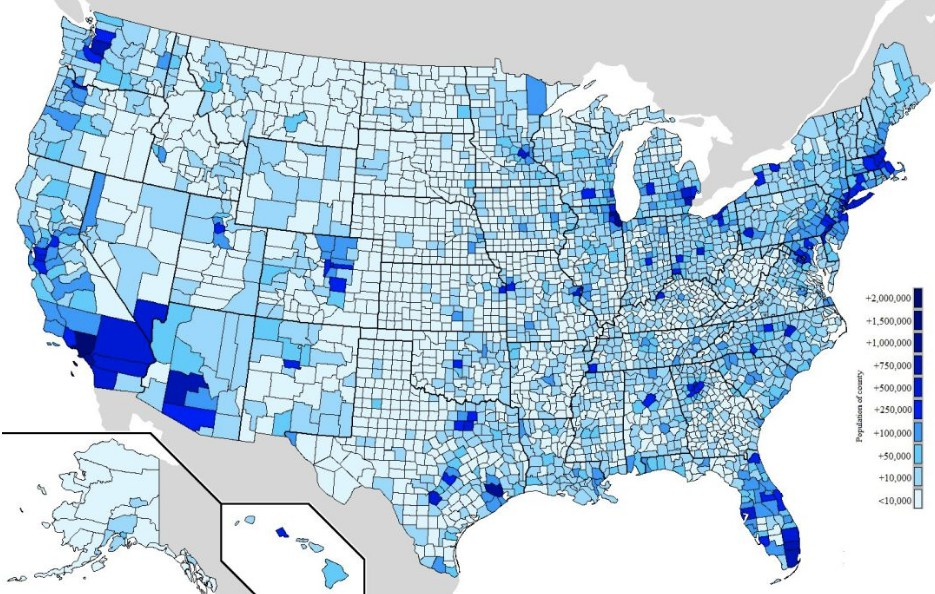
\includegraphics[width=.9\textwidth]{US_Population.jpg}
	\caption{The population density of the US}\label{fig:1}
\end{figure}	

	\item \textbf{The number of car ownership}
	
We analyzed car ownership in the United States over the last 12 years. The population growth is plotted as Figure \ref{fig:2}, According to the figure, we observe that the number of cars ownership is linear with the year. So we use linear fitting to analyze the number of cars ownership.We use the function
$f(x) = {p_1}x + {p_2}$ to match the growth. By fitting, we get the car ownership ${C_{car}}$ for the next five years.
\begin{figure}[H]
	\centering
	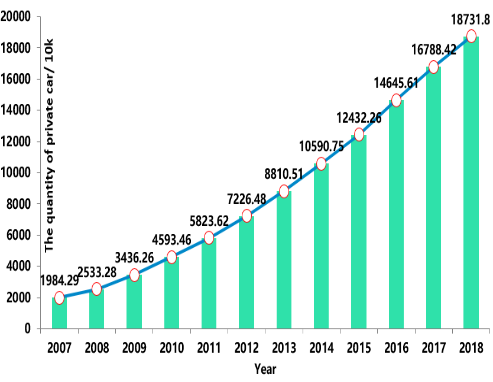
\includegraphics[width=.6\textwidth]{US_Car_Increase.png}
	\caption{The ownership of car in US}\label{fig:2}
\end{figure}

	\item \textbf{The number of charging stations}
	
Similar to above, by searching for data we finally find the growing distribution of Tesla charging stations over the past few years. Through analysis, we find that the distribution of Tesla charging stations presents a quadratic relationship in years.So we use fuction $f(x) = {p_1}{x^2} + {p_2}x + {p_3}$ to match the growth. By fitting with matlab, we also predicted the growth trend of Tesla charging stations in the next five years(${p_1=196.9, p_2=1535, p_3=1555}$).
\begin{figure}[H]
	\centering
	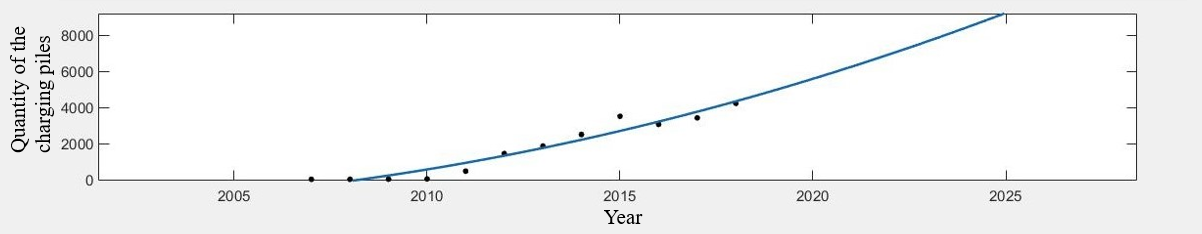
\includegraphics[height=.11\textheight]{tesla_station.png}
	\caption{The number of Tesla charging stations}\label{fig:3}
\end{figure}

\end{itemize}

\subsection{All-electric analysis model}
\subsubsection{The model construction}
\textbf{1. Advanced queuing theory model $M/M/1/\infty $}

In our model, a charging station can be viewed as a server in queuing theory, through the queuing theory model $M/M/1/\infty $ and our prediction, we can analyze the station's intensity of the service $\rho $ and the average waiting time ${W_s}$ . 
Firstly, according to the distribution of cars growth in the United States and the land area of the US, we define the parameter ${f_d}$. That's the number of cars per person in the United States.
\begin{equation}\label{eq:fd}
{f_d} = \frac{C_{car}}{S}
\end{equation}

And we define the parameter $k$ to be the percentage of cars that are electric. 
We assume that the number of cars arriving at the charging station obeys the possion distribution with the parameter $\lambda $. Suppose a car is charged once a week, we got:
\begin{equation}\label{eq:lambda}
\mathop \lambda \limits^ \wedge   = \frac{{C_{car} \times k}}{{S \times 168}}
\end{equation}

At the same time, we assume that the service time of charging stations obeys negative exponential distribution with the parameter $\mu $. Consider that there are two different charging stations: super charging stations and destination charging stations. We assign them different weights to represent service hours, so we got:
\begin{equation}\label{eq:mu}
\mathop \mu \limits^ \wedge   = \frac{{{C_{des}} \times {t_{des}} + {C_{\sup }} \times {t_{\sup }}}}{S}
\end{equation}

Based on what we've assumed, when the vehicle arrives at the charging station at a possion, if at this time there are a number of vehicles are charging, then the vehicle must wait in line, so we can get the intensity of the service $\rho $ , the average waiting time ${W_s}$ and the average waiting captain as follows:
\begin{equation}\label{eq:queue}
\begin{array}{l}
\rho  = \frac{\lambda }{\mu }\\
\\
{L_q} = \frac{{{\rho ^2}}}{{1 - \rho }}\\
\\
{W_s} = \frac{1}{{\mu  - \lambda }}
\end{array}
\end{equation}

Give the parameter $\mu $ and $\lambda $ , we can analyze them by our model and finally receive the intensity of the service $\rho $.

\textbf{2. Two-objective programming to minimize the waiting time and station quantity}

Based on the assumptions from the problem, the all-electric has come true. So we can define the parameter k=1. From the concepts statements above, we have divided the United States by population density. We can apply our queuing model to the urban, suburban and rural areas. According to the problem, we are asked to give the quantity of the charging stations and their distribution. So we introduce two-objective programming model to minimize the charging stations with the lowest average waiting time, according to our calculations, when the average waiting time is lower than 1 hour, we think the quantity of the stations can meet the demand. 
Our target: 
\begin{equation}\label{eq:tar}
\left\{ {\begin{array}{*{20}{c}}
	{\min \left\{ {{Q_{ur}} + {Q_{su}} + {Q_{ru}}} \right\}}\\
	{}\\
	{\min \{ {\rho _{ur}} + {\rho _{su}} + {\rho _{ru}}\} }
	\end{array}} \right.
\end{equation}

The ${Q_{ur}}$, ${Q_{su}}$,and ${Q_{ru}}$ respectively represent the quantity of the stations of the urban, suburban and rural areas.
In order to find out the restrictions, we define parameter ${t_{per}}$ to express the charging time per car. And define parameter ${C_{per}}$ to express the charging cars per day. Based on this, we finally give our restrictions of the two-objective programming model:
\begin{equation}\label{eq:restrict}
s.t\left\{ {\begin{array}{*{20}{c}}
	{\sum {{C_{per}}}  \times {t_{per}} \le \sum {{W_s}} }\\
	{{Q_{ur}} + {Q_{su}} + {Q_{ru}} \ge \frac{{{C_{per}} \times {t_{per}}}}{{\mathop \mu \limits^ \wedge  }}}\\
	\begin{array}{l}
	{\rho _{ur}} + {\rho _{su}} + {\rho _{ru}} = 1\\
	{\rho _{ur}},{\rho _{su}},{\rho _{ru}} > 0
	\end{array}
	\end{array}} \right.
\end{equation}

\subsubsection{Model solution and analysis}
By solving the model above, we get clear results below:

1. According to the current growth trend of electric vehicles and charging stations, Tesla is not able to provide basic charging services under the condition of complete switch to electric vehicles in the United States.
According to our model, when the proportion of electric vehicles ${k}$ reaches 1, the avarage waiting time ${W_s}$ is calculated to be 5.32 hours according to the queuing theory model greatly exceeds the acceptable waiting time range of charging, so it's reasonable to think that Tesla can not meet the basic living needs of the people in future time.

2. According our definition of urban, suburban and remote areas based on population density, we have the relevant parameters such as work intensity and average waiting time obtained by queuing theory model.
Considering the load of power, we reasonably limit the sum of work intensity of charging stations in urban, suburban and rural areas to  equal to 1,\ ${(\rho _{ur} + {\rho _{su}} + {\rho _{ru}} = 1)}$. In addition, according to the total charging time less than the total waiting time
${(\sum {{C_{per}}}  \times {t_{per}} \le \sum {{W_s}}) }$
, all parameters are positive\ ${({\rho _{ur}},{\rho _{su}},{\rho _{ru}} > 0)}$\ , we get the corresponding constraints.
by combining the expression with the constraints, we have the optimal ratio of the number of urban, suburban and remote areas charging stations,\ ${3.23:1.07:0.34 }$, and the total quantity of charging stations is 16025, therefore we get the exact number of each charging station.
\begin{table}[H]
\begin{center}
\caption{Quantities of charging stations in US}
\begin{tabular}{cccc}
	\toprule
	Location of charging station & Urban & Suburban & Rural areas\\
	\midrule
	Quantity & 11162 & 3698 & 1175\\
	\bottomrule
\end{tabular}\label{tb:2}
\end{center}
\end{table}

\section{Exploring charging network in South Korea}
\subsection{Charging station distribution model}
\subsubsection{Using our previous model in South Korea}

From what we have discussed on task 1, firstly we use our model to analyze the exact quantities of charging stations in South Korea. Korea is one of the typical country in the world which have the ability to complete the plan of replacing motor vehicles with electric cars. By running our model on Matlab, we finally get the answer:
\begin{table}[H]
\caption{Quantities of charging stations in South Korea}
\begin{center}
	\begin{tabular}{cccc}
		\toprule
		Location of charging station & Urban & Suburban & Rural areas\\
		\midrule
		Quantity & 5812 & 2297 & 432\\
		\bottomrule
	\end{tabular}\label{tb:3}
\end{center}
\end{table}
\subsubsection{Station quantity model}

When it comes to the quantitive selection of charging stations, we analyze the urban distribution in South Korea and finally find a quantity model.

\begin{figure}[H]
	\centering
	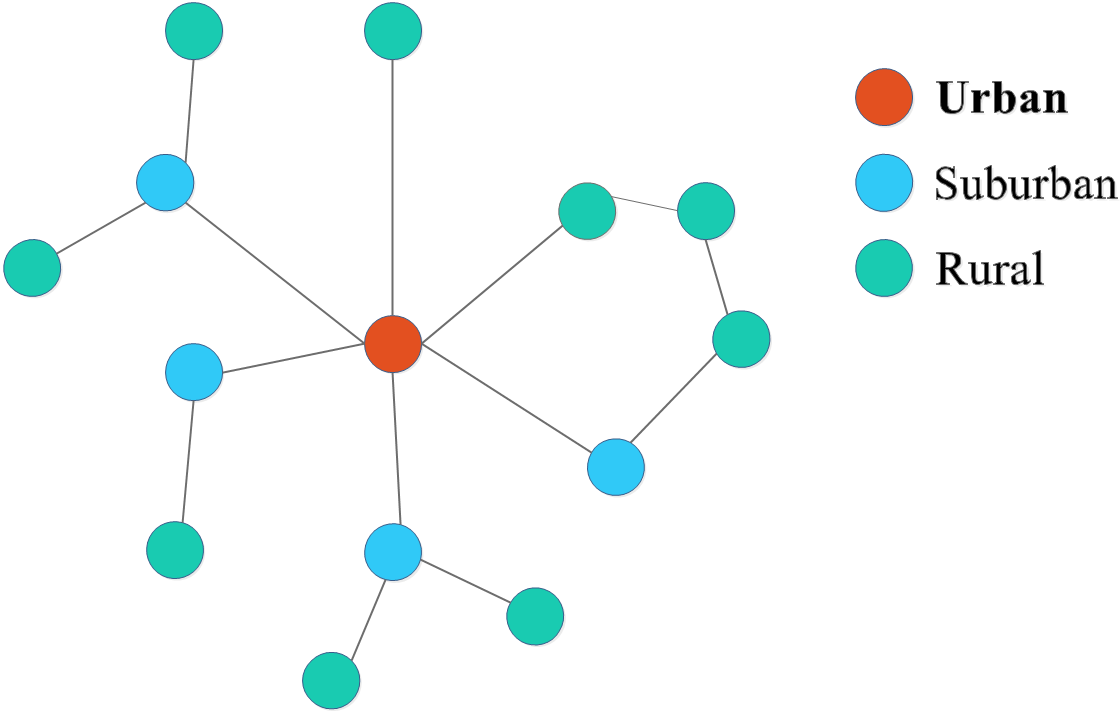
\includegraphics[width=.6\textwidth]{Net.png}
	\caption{The transportation network with urban,suburban and rural area}\label{fig:4}
\end{figure}

We take each town as the node and the road between the towns as the edge, forming an undirected topology. Then we take the road between two nodes as the object of discussion. By analyzing how many charging stations are needed for each road. Hence we got the total stations needed in South Korea.

\begin{itemize}
	\item We assume that the $g$ refers to the electric vehicle power consumption. Because there are so many different kinds of electric vehicles, we define ${g_k}$ for different kinds.
	\item We assume that the $q(x)$ refers to the traffic flow with the unit car / h , since we want to discuss the flow in a section of the road. We define $q(x,k)$ for the k-type electric vehicle's flow in the x-section of the road.
	\item We assume that the $V(L)$ refers to the power consumption on the road L, with the unit W / day.
\end{itemize}

And our model as follows:

First, we can figure out the k-type of the car's power consumption on the i-section of the L-road $V(i,k)$ \cite{3}:
\begin{equation}
V(i,k) = g(k) \times L(i) \times q(i,k)
\end{equation}

Then we can get the all kinds of cars's power consumption on the i-section of the L-road:
\begin{equation}
V(i) = L(i) \times \sum\limits_{k = 1}^M {V(i,k)}
\end{equation}

Finally, we can figure out the total power consumption of the L-road:
\begin{equation}
V(L) = \sum\limits_{i = 1}^N {V(i)}
\end{equation}

We define $P$ for the power that one charging station can give per day. Here we can assume two types of the P as $P_s$ for super-charging station and $P_d$ for destination-charging station. So we can get the final number of the charging stations $N$:
\begin{equation}
N = \frac{{V(L)}}{P} = \frac{{\sum\limits_{i = 1}^N {L(i) \times \sum\limits_{i = 1}^M {g(k) \times q(i,k)} } }}{P}
\end{equation}

\begin{figure}[H]
	\centering
	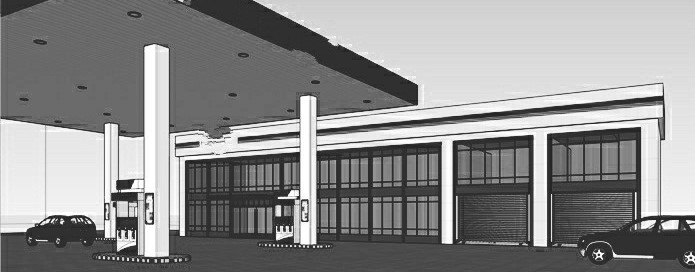
\includegraphics[width=.8\textwidth]{charging_station.jpg}
	\caption{The charging station}\label{fig:5}
\end{figure}

\subsubsection{Station position model}
From the Station quantity model, we can get the number of stations needed in every road of the South Korea's transportation network. However, from that model we can not accurately allocate each station. So we introduce our station position model to solve the distribution problem. 

Firstly, we analyze the population and average daily passing vehicle between two kinds of areas. We hold the opinion that there are two conditions would lead the high-flow of the cars: the one is near the urban area and the other is near the transportation junction. Here are the analysis graphics:

\begin{figure}[H]
	\centering
	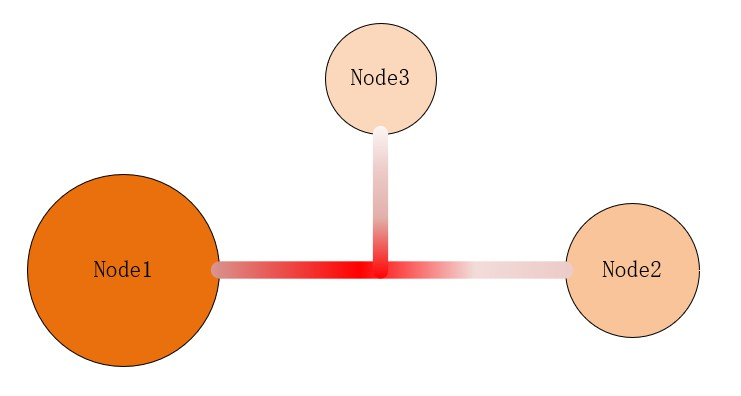
\includegraphics[scale=0.7]{Node_flow.jpg}
	\caption{The traffic flow among the nodes}\label{fig:6}
\end{figure}

Consider both flow and distance, here are our model:
\begin{itemize}
	\item site the $q(x)$ above to measure the x-position's traffic flow.
	\item define $d(x,i)$ to measure the distance between the x-position and node i. 
\end{itemize}

And our model is to find out the x-position that meet the conditions that let the $q(x)$ to be the highest and simultaneously minimize the $d(x,i)$ :

\begin{equation}
\left\{ {\begin{array}{*{20}{c}}
	{\max \{ q(x)\} }\\
	{}\\
	{\min \{ \sum\limits_{i = 1}^n {d(x,i)\} } }
	\end{array}} \right.
\end{equation}

Where $n$ represents the number of nodes.

By looking up for information we finally divite the areas in South Korea into the urban node, suburban node, and rural node depends on the density of the population. By using our station quantity model and station position model, we solved our models and give an analysis of the distribution of South Korea. In figure 7, we can find the urban area with the color red, the suburban area with the color blue and the rural area with the color green.
\begin{figure}[H]
	\centering
	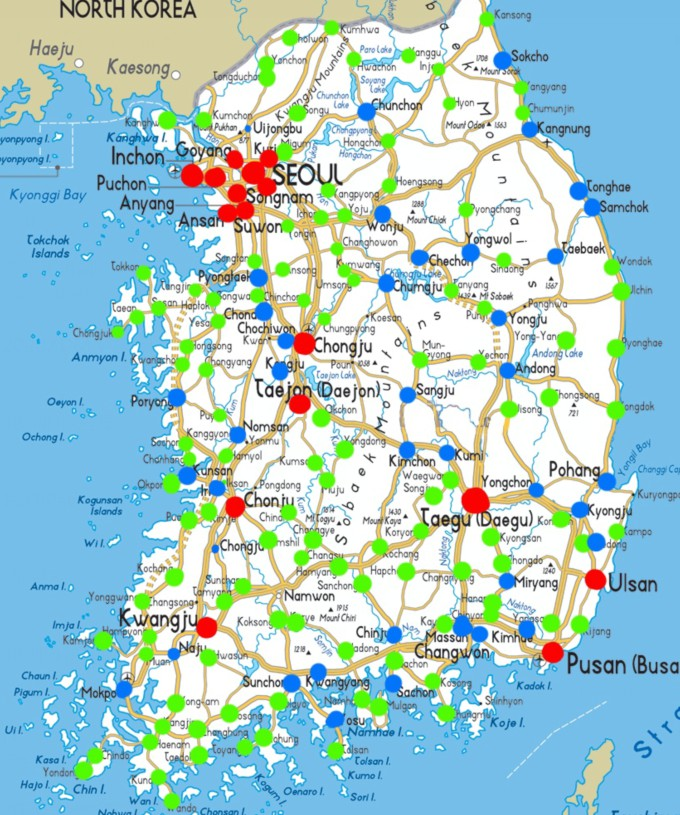
\includegraphics[width=.5\textwidth]{Korea_cities.jpg}
	\caption{Korea traffic node allocation}\label{fig:7}
\end{figure}
\begin{figure}[H]
	\centering
	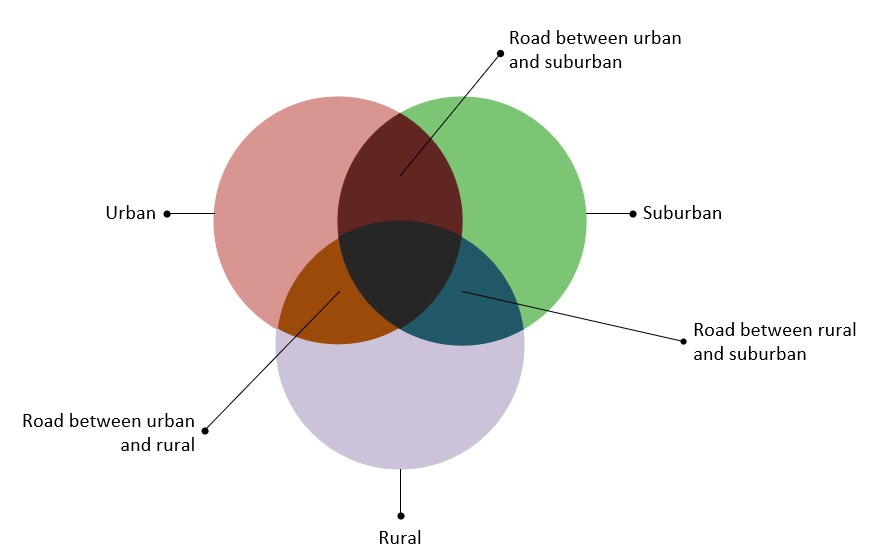
\includegraphics[scale=0.7]{road.jpg}
	\caption{Three kinds of roads}\label{fig:8}
\end{figure}
\subsubsection{Model solution and analysis}
By solving our model above, first we find 5 different roads in South Korea and got their traffic flow by 3 different types of cars. According to the hypothesis, we assume these cars are 3 types of electric cars. From the left to right we call the road for roadA to roadE. 
\begin{figure}[H]
	\centering
	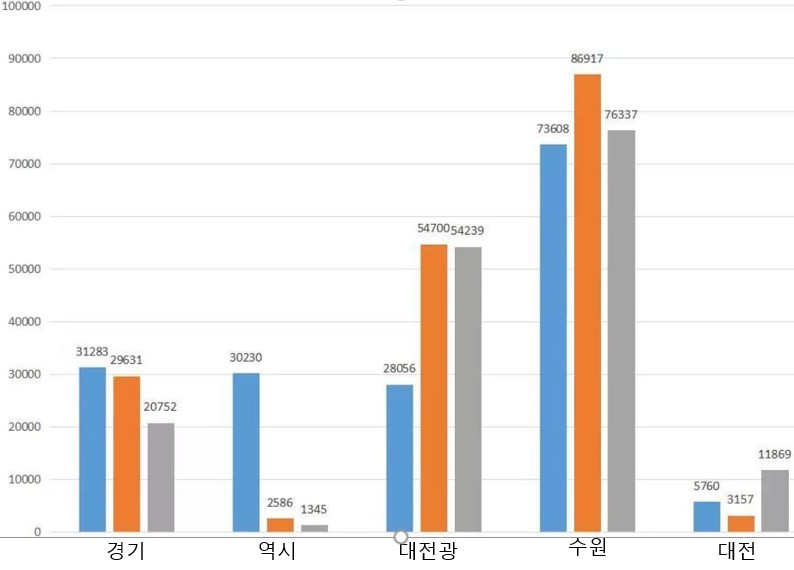
\includegraphics[width=.8\textwidth]{traffic.jpg}
	\caption{The traffic flow on the road}\label{fig:9}
\end{figure}

By running our model on matlab, we can get the exact number of stations needed for each road. 
\begin{table}[H]
	\caption{Quantities of charging stations in each road}
	\begin{center}
		\begin{tabular}{cccccc}
			\toprule
			road & roadA & roadB & roadC & roadD & roadE\\
			\midrule
			Quantity & 10 & 5 & 14 & 33 & 3\\
			\bottomrule
		\end{tabular}\label{tb:4}
	\end{center}
\end{table}

According to the data, we can give an estimation that when it comes to the all-electric, there are about 18200 charging stations are needed. And consider to the two different types of charging piles, we assume that the super charging piles are installed in the long-distance road like urban-urban road, and the destination charging piles are mainly installed in the areas.
\begin{figure}[H]
	\centering
	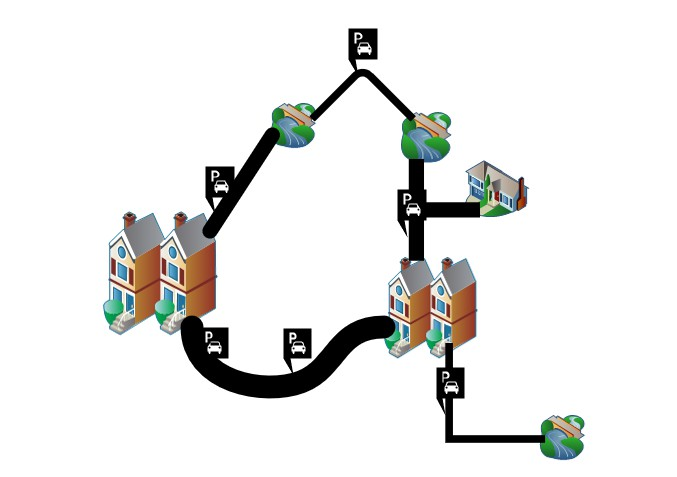
\includegraphics[scale=0.6]{urban_to.jpg}
	\caption{Simulation of the distribution}\label{fig:10}
\end{figure}
\subsection{The priority of construction}

According to the intent, there are three options.
\begin{itemize}
\item Build a better network of charging piles before attracting consumers to buy EVs.
\item Provide preferential policies first to attract customers to purchase a large number of EV before building a charging network.
\item To first build a basic network and then the basic network will promote the purchase of electric vehicles.
\end{itemize}

Option 1 has extremely high requirements for capital flow, and the charging piles built in the early stage have sunk costs because they are not used by users;
Option two, there may be a good sales volume in the early stage, but the growth rate is slowed down because the number of charging piles is difficult to meet the user's growth demand, and the capital flow is not flexible.

The third option is our best choice. We can first build a basic charging station network with less funds to meet the most basic needs of the initial users, which will reduce the initial capital investment without adversely affecting subsequent growth. The corresponding quantitative analysis and distribution is shown in the next question.
\subsection{Maximum Spanning Tree Based on Optimized Potential Model}
We can start with a clean slate, therefore, a maximum spanning tree model based on improved reachability weights can be introduced to solve the problem.
\begin{itemize}
	\item Basic potential model
\end{itemize}

Where\ ${M_j}$\ represents the quality of activity at point j, and\  ${D_{ij}}$\  represents the travel impedance factor (distance or time) between points i and j.
In a system, the potential energy generated by all objects at a point is equal to the sum of the potential energy generated by each object at that point.For example, there are n discretely distributed objects in space, the exaggrat potential ${A_i}$ meets the equation blow\cite{2}.
\begin{equation}
		A_{i}=\sum\limits_{j=1}^{n} A_{i j}=\sum\limits_{j=1}^{n} \frac{M_{j}}{D_{i j}}
\end{equation}
\begin{itemize}
	\item Modified potential model applicable to this problem
\end{itemize}

Let \ ${M_j}$\  be a constant that is positively related to population density, average income and employment rate (We can use Urban Development Index to quantify ${M_j}$),\  ${C_{ij}}$\  is the direct distance between i and j, and a is the distance friction constant. Then we have a new equation.
\begin{equation}
	P_{i}=\sum_{j=1}^{n} \frac{M j}{C_{i j}^{a}}
\end{equation}

The potential value of each point was calculated according to the formula, the two-point potential and / distance were used as the weight between nodes, and the modified prim algorithm was used to obtain the maximum generation number and node sequence. The node sequence was used as the basis for the construction order of charging stations.

It should be noted that the choice of the travel friction coefficient ${\alpha}$, on the one hand, ${\alpha}$ can be selected different values for different applications, which improves the accuracy of such model evaluation and expands the scope of application, but on the other hand ${\alpha}$ Therefore, the value of is a difficult problem. After consulting a large amount of paper, we get the ideal value of ${\alpha}$ which is 1.85\cite{1}.

From this, an ordered node set can be obtained, and the corresponding ordered edge set ${E}$ is obtained according to the ordered nodes.It is assumed that the funds ${C}$ used for the construction of the charging station is constant every year, given that South Korea is already a developed country, and the country's economic growth has slowed down. Therefore, it's reasonable to assume that the total number of private cars remains the same and the total number of charging piles ${Q}$  remains unchanged. 

According to the above number and distribution model, we can get the optimal number of charging stations between each node, and their distribution which means we have ${K_{ij}}$ represents the optimal number of charging stations between ${i}$ and ${j}$ nodes obtained from the previous model, and ${f}$ represents the funds required to build a gas station. Above all, we have the n-year electric vehicle market share ${m}$ starting from 2020 as the first year${(i,j\ in \ edge\  set\  E)}$.
\begin{equation}
m = \sum\limits_{i = 1}^n {\frac{C}{{ K_{ij} \times p*Q}}} 
\end{equation}

Plug in the data, running our model on matlab and we finally plot the Electric-Veicle ratio development in South Korea as follow: 
\begin{figure}[H]
	\centering
	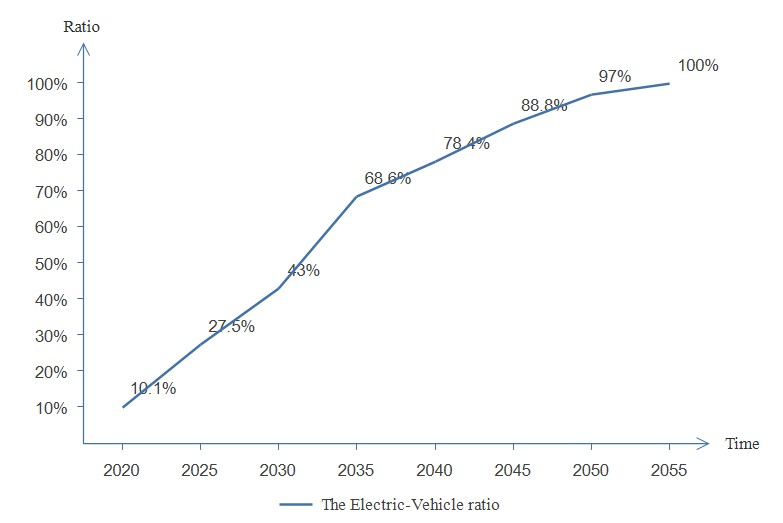
\includegraphics[scale=0.8]{time.jpg}
	\caption{The Electric-Vehicle ratio}\label{fig:11}
\end{figure}

\section{IP Model for Classification System }
Now we can have a overview about countries with different regions, population density distributions and wealth distributions, such as Australia, China, Indonesia, Saudi Arabia, and Singapore.

From economic principles we can know the following two obvious facts
\begin{itemize}
	\item The regional population density is defined as ${\rho}$, and the wealth distribution is measured by the regional per capita income ${y}$. Then it is obvious that the development of the electric vehicle market needs to be extended from economically developed regions to extended economically backward regions. The purchasing power of residents in economically developed regions is significantly higher than in economically backward regions Under the same market conditions, the consumption power is higher, which will promote the development of the electric vehicle market.
	\item Since electric vehicles have almost the same endurance capacity as traditional cars during short-term driving, this effect is not considered in the short range. When rolling out the electric vehicle network, we should consider interconnecting in economically developed areas, and then proceed to economically backward areas in turn. For long-term driving charging needs, when constructing a charging pile network, attention should be paid to the construction of an intermediate station charging network between two isolated points to meet consumer needs.
\end{itemize}

Therefore we have the IP Model\ (Income-Population Model) to classify different countries. In our model we have two basic assumptions:

1. The frequency of residents using electric vehicles in a certain area is positively related to the population density in the area. After the electric vehicle network covers the area, the distribution of charging piles for electric vehicles should match the population density distribution.

2. Regional per capita income is related to the consumption of electric vehicles and will also affect the network configuration of electric vehicle charging devices. The number of per capita charging piles in the area is related to their per capita income. We introduce population coefficient ${\rho}$ and income coefficient ${\psi}$ to evaluate the degree of imbalance.
\begin{equation}
	\varphi  = {\textstyle{{\sqrt {\frac{1}{n}\sum\limits_{i = 1}^n {{{({\rho _i} - \overline \rho  )}^2}} } } \over {\overline \rho  }}}\
\end{equation}
\begin{equation}
	\psi  = \frac{{\sqrt {\frac{1}{n}\sum\limits_{i = 1}^n {{{({y_i} - \overline y )}^2}} } }}{{\overline y }}\
\end{equation}

According to our model, we can get demographically balanced and economically balanced countries, we regard a country as a unbalanced country if it's demographically unbalanced or economically unbalanced, otherwise it's a balanced country.

\begin{figure}[H]
	\centering
	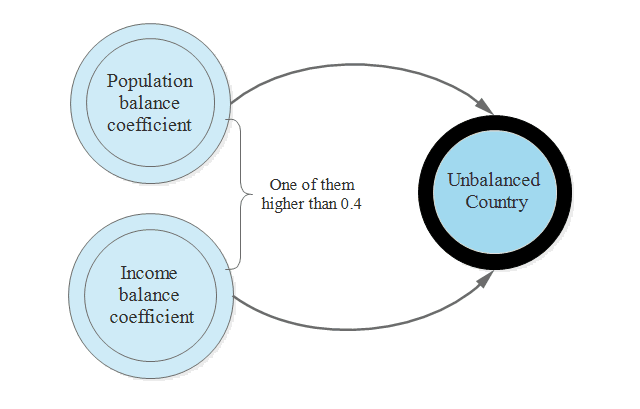
\includegraphics[scale=0.5]{Judge.png}
	\caption{Way to judge if a country is a balanced country}\label{fig:12}
\end{figure}

We introduce the Gini coefficient to evaluate our model, to judge whether the country's economic development is balanced or not is a major criterion for economic evaluation of our team. According to international standards, the warning line for the Gini index is set to 0.4. It is considered as an imbalanced economic development, rich and poor The gap is clearly defined.

According to our model:

 China, Russia, Indonesia, Saudi Arabia, and Singapore are considered imbalanced countries. 
 
 The United States, South Korea, Ireland, Germany, Uruguay, and Japan are balanced countries. 
\begin{figure}[H]
	\centering
	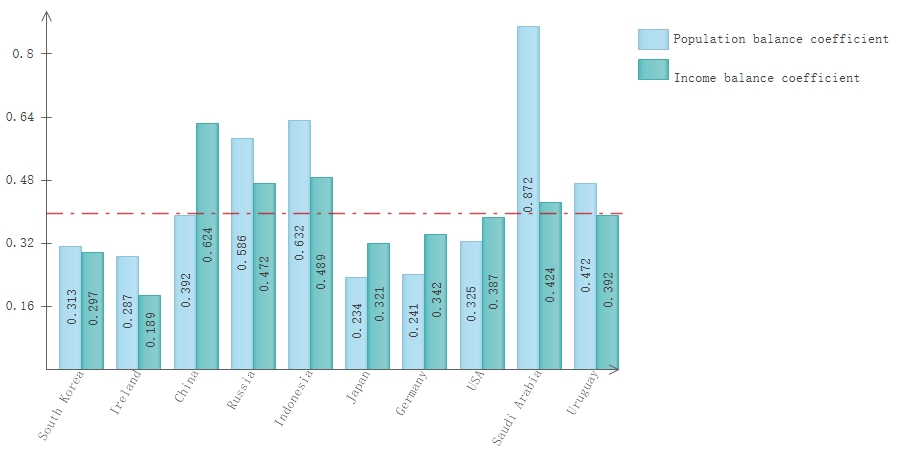
\includegraphics[scale=0.6]{Country.jpg}
	\caption{Coefficient ${\rho, \psi}$ of each country}\label{fig:13}
\end{figure}
Via Gini coefficient, we get:

Balance countries: South Korea, Ireland, Japan, Germany, United States

Imbalanced countries: China, Russia, Indonesia, Saudi Arabia, Uruguay
The following is the Gini index of each country.
\begin{figure}[H]
	\centering
	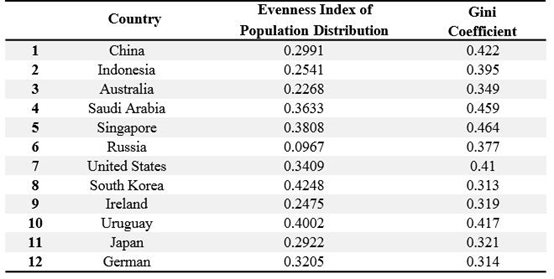
\includegraphics[scale=0.6]{kini.png}
	\caption{Gini Coefficient of each country}\label{fig:14}
\end{figure}

So we have two plans.

1. For balanced country
Construction of charging piles is being carried out in all regions at the same time. Although most groups will use the system at the same time to promote long-term stable and gentle growth, it will promote most of the development as a whole and provide differentiated services based on market surveys. Market pricing is basically the same.

2. Targeting developing countries
Developed areas are prioritized to roll out charging pile equipment. At the same time, the charging price when building charging piles in economically backward areas can be lower than in developed areas, reducing some profits and winning new consumers. At the same time, charging piles developed in different economic levels Installations should be differentiated in quantity. Based on the principle of "prioritizing developed areas, profit first, remote areas, and customers later," they occupy the urban market first and then expand the rural market.

\section{Competitive model for new technology}

For the new technology such as car-share and ride-share services, self-driving cars, rapid battery-swap stations for electric cars, flying cars and Hyperloop. We establish our competitive model through its objective influence, subjective influence and the development of the technology.

We define:
\begin{itemize}
	\item ${\theta _i}$ for technology-i's development index.
	\item ${e_i}$ for the technology-i's promotion and restriction level.
	
	The ${e_i}$ includes two kinds of index:
	
	${\alpha _i}$ for the objectivity of technology itself, it is mainly determined by the technology's competitive relation with the electric-vehicle development. And its value is 1 or -1.
	
	${\beta _i}$ for the subjectivity of people's willingness, it is mainly determined by the convenience and the price of the technology.
\end{itemize}

\begin{figure}[H]
	\centering
	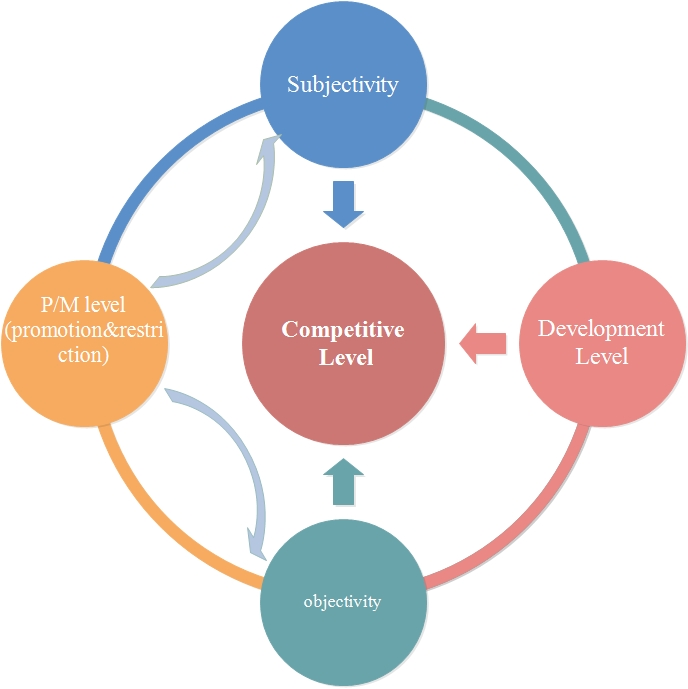
\includegraphics[scale=0.5]{Task4.jpg}
	\caption{Competitive Model}\label{fig:15}
\end{figure}

Through our collection of data and personal rating, by analytic hierarchy process and normalized factor finally we obtain the total competitive level $f(i)$ for each technology.

\begin{equation}
f(i) = {\theta _i} \times {e_i} = {\theta _i} \times {\alpha _i} \times {\beta _i}
\end{equation}


\begin{table}[H]
	\caption{competitive level for each tech}
	\setlength{\tabcolsep}{8mm}
	\begin{center}
	\begin{tabular}{cccccc}
		\toprule[2pt]
\textbf{Name of new technology}                                                                 & \textbf{${\theta _i}$} & \textbf{${\alpha _i}$} & \textbf{${\beta _i}$} & \textbf{f(i)} \\ \hline
\textbf{car-share}                                                                              & 0.85                   & -1                     & 0.70                  & -0.595        \\ \hline
\textbf{ride-share services}                                                                    & 0.73                   & -1                     & 0.62                  & -0.4526       \\ \hline
\textbf{self-driving cars}                                                                      & 0.47                   & 1                      & 0.37                  & 0.1739        \\ \hline
\textbf{\begin{tabular}[c]{@{}l@{}}rapid battery-swap station for\\ electric cars\end{tabular}} & 0.37                   & 1                      & 0.43                  & 0.1591        \\ \hline
\textbf{flying cars}                                                                            & 0.13                   & 1                      & 0.26                  & 0.0338        \\ \hline
\textbf{hyperloop}                                                                              & 0.29                   & -1                     & 0.62                  & -0.1798        \\ 
		\bottomrule[2pt]
	\end{tabular}
\end{center}
\end{table}

According to our model, we can figure out that the car-share, ride-share services and hyperloop have the negative impact on the development of electric-vehicle development, and the self-driving cars, rapid battery-swap station for electric cars and flying cars have the positive impact on the development of electric-vehicle development. The result fits our perception because share-economy will definitely reduce the sales of cars including electric cars. For the advanced technology, in view of their slow state of development, as opposed to rapidly developing electric-vehicle, it will have less impact.


\section{Sensitivity Analysis}
We have conducted a sensitivity analysis of the All-electric analysis model.

For the parameter $t_{per}$: charging time for single car is an uncertainty. We analyzed its sensitivity, giving the $t_{per}$ for range [0.5,8] and calculating the number of charging stations required, finally get our conclusion:

It doesn't matter how long a car takes to charge, the number of the stations stays stable. So the parameter $t_{per}$ isn't a sensitive parameter.

\begin{figure}[H]
	\centering
	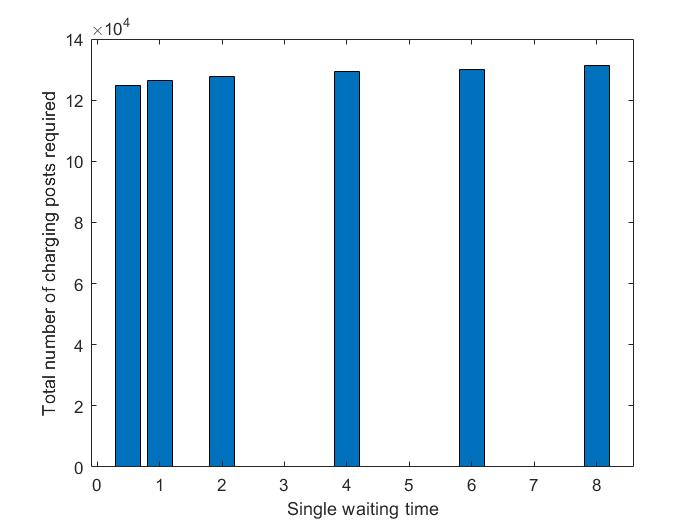
\includegraphics[scale=0.4]{average.jpg}
	\caption{Sensitivity of the $t_{per}$}\label{fig:16}
\end{figure}

For task 2, we also conducted a sensitivity analysis of our Station quantity model. We assume that the traffic flow is the sensitive parameter for the quantity of the charging station. By changing the daily vehicle flow of the Road A and with our two-objective programming model we finally get the number of stations' changing situation as follow:

\begin{figure}[H]
	\centering
	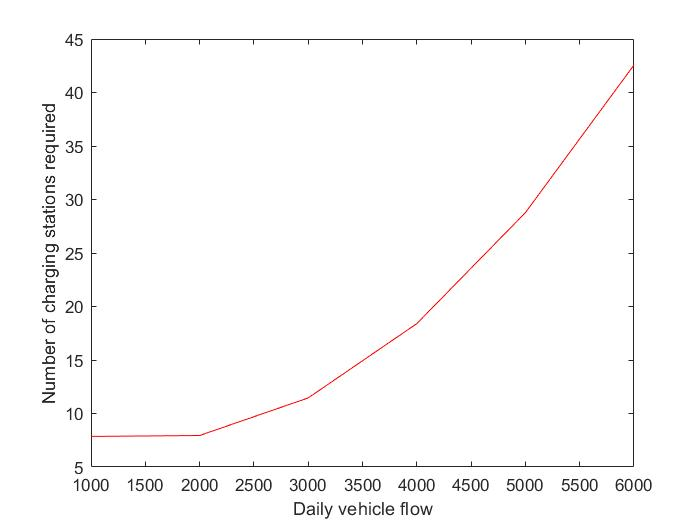
\includegraphics[scale=0.4]{vehicle.jpg}
	\caption{Sensitivity of the traffic flow}\label{fig:17}
\end{figure}

It's easy to see that with the changing of the daily vehicle flow, the number of changing stations required has a rapid change. So we give the conclusion that the traffic flow is a sensitive parameter.



\section{Strengths and Weaknesses}
\begin{itemize}
	\item Covering many fields like  engineering, management, statistics and economy enables the paper to study the question from the big picture which makes our model comprehensive and precise.
	\item For the quantity model in task 1, we classified urban, suburban and rural areas based on the population density in U.S. which makes the question clear and simple
	For the quantity model in task2a, we creatively applied the relationship between the vehicle power consumption and the charging capacity provided by the charging stations and therefore greatly simplified the problem with little loss in reliability.
	\item For our site-selection model and construction plan we innovatively introduced potential model in accessibility research in the calculation of edge weight and improve it by redefining the coefficient ${M_j}$ to the development index covering economy, population, transportation and future development which makes the model more universal and robust.
\end{itemize}

\subsection{Weaknesses}
\begin{itemize}
	\item Due to time and data constraints, the model fails to considerate the differences within different distribution of the super-charing piles and destination charging piles.
	\item The sources of data are not wide enough so that models are difficult to solve effectively. However, the optimality of the models are always established, in other words, the model always solves the correct optimal result based on the given data. 
\end{itemize}


\clearpage
\section{Handout}
\begin{center}
	\textbf{Handout for the leader}
\end{center}

Welcome to the international energy summit!

It’s a great honor for us to present you our research results of the migration towards electric vehicles. We sincerely hope that it will provide some references for you while making policies and plans. We also hope our suggestions could play a part in the development of electric vehicles and the betterment of human development. In the next part of the handout, we will describe our modeling concepts and advice to you in detail.

The key factors of our model include: population density, degree of economic development, user density and the level of traffic flow,and traffic accessibility, which can be quantified precisely. Other factors include geographies, consumer psychology or other factors that are hard to quantify.

The components and functions are listed in our article in detail. You can refer to them while formulating policies. In our model, there are three steps for you to finally confirm your plan for the gas vehicle-ban.

Firstly, use the queuing model based on the population density and car ownership to minimize the quantity of the charging stations and the average intensity of the service. Combine with the development in your country you can finally roughly determined the number of the charging stations in the area.

Secondly, according to the country’s transportation network, with the data of the traffic flow, you can confirm the exact number of the charging stations on the road between one area and another area. Then with our station position model you can determine the position of the stations and confirm the distribution in the end.

Then, with the maximum spanning tree modified potential model, according to the degree of the economic development and the accessibility, you can determine the sequence of charging stations and finally get the timeline of the all-electric degree.

By using the methods we provide, you can also estimate the exact time when electric vehicles is in certain proportion to traditional vehicles. According to the timetable, a gas vehicle-ban date can be decided scientifically.

Since each country has its specific situation, there will be some inevitable errors and uncertainties in our model, but it can provide a general development forecast for different countries to better achieve the full coverage of electric vehicles, I hope our model can benefit your country to some extend, thank you for coming to this summit.

Best wishes!
% 参考文献,此处以 MLA 引用格式为例
\clearpage
\begin{thebibliography}{99}
\bibitem{1} 
Zhengna Song, Wen Chen.Evaluation method of spatial accessibility of medical facilities based on potential model.[J].\emph{Progress in geosciences},2009,28(06):848-854.
\bibitem{2} 
Pinghua Li, Yuqi Lu.Review and Prospect of Accessibility Research[J].\emph{Progress in geosciences},2005(03):69-78.
\bibitem{3}
Ma Yifei, Gao Rongxiao. Gas station layout model for road section [J]. \emph{Operations Research and Management Science}, 2005 (5): 63-68.
\bibitem{4}
Tian Naishuo. N-Strategy CI / M / 1 Random Service System [J]. \emph{Mathematics in Practice and Theory}, 1992 (01): 29-35.
\bibitem{5}
Kim K , Kahng B , Kim D . Jamming transition in traffic flow under the priority queuing protocol[J]. \emph{EPL (Europhysics Letters)}, 2009, 86(5):58002.
\bibitem{6}
Tian Wang.Building Charging Network for Electric Vehicles in Automobile Supply Chains[D].\emph{Huazhong University of Science and Technology},2015.
\end{thebibliography}


\end{document}  % 结束